\chapter{Signal Analysis}
\paragraph{}  The large number of sensors and the rapid sampling of each sensor provides an enormous number of individual measurements of magnetic fields during the plasma's lifetime. The method of Biorthogonal Decomposition is used to isolate coherent fluctuations from this large dataset and provides an orthogonal basis set of modes, that are described in terms of their spatial shape and temporal evolution.  This chapter will describe the method of Biorthogonal Decomposition, how it is applied in this research, its strengths and limitations.

\section{The Biorthogonal Decomposition Algorithm}
\paragraph{}
The biorthogonal decomposition is used on non-square matrices, to produce a basis set of pseudo-eigenvalues and pseudo-eigenvectors.  A given matrix S is decomposed into 
\begin{equation}
S^{\intercal} S = U \Sigma V^{\intercal}
\end{equation}
Where the columns of U and the rows of V are orthogonal bases of the structures, however defined, that make up the rows and columns of the data. In this research, the rows are time series of individual sensor signals, with the signal across all sensors at any instant constituting the columns.  
$$
\begin{pmatrix}
\uparrow& &\uparrow\\
s_1&\cdots&s_N\\
\downarrow & &\downarrow
\end{pmatrix}
 =
\begin{pmatrix}
\uparrow& &\uparrow\\
u_1&\cdots&u_N\\
\downarrow & &\downarrow
\end{pmatrix}
\begin{pmatrix}
\sigma_1& &\\
&\ddots&\\
& &\sigma_N
\end{pmatrix}
\begin{pmatrix}
\leftarrow& v_1&\rightarrow\\
&\vdots&\\
\leftarrow& v_M &\rightarrow
\end{pmatrix}
$$



  can be derived by first multiplying the vector by its transpose.  The resulting matrix is square and is factorable into two independent sets of eigenvectors, which are related to the arrangement of column and row vectors.  
In the case of HBT-EP, the time-domain signal for each sensor is stitched together to give a matrix that has dimensions up to 216 X 5000.  The set of eigenvalues will be equal in size to the smaller dimension.  \par
The set of eigenvectors will be determined arbitrarily, with no a priori assumptions as to the form of the basis functions.  The only constraint is that they must all be orthogonal in both space and time.  That the poloidal modes do not form a clean Fourier basis set is therefore of no concern.  The toroidal and temporal structure, for which sinusoids are a good description, will allow for orthogonal bases which map well onto individual modes regardless of poloidal structure.  Thus modes with non-singular poloidal spectra can be well modeled, which would not be the case if a Fourier basis was imposed.\par
A set of synthetic data is generated and analyzed with the biorthogonal decomposition to show the utility of the method.  The plasma current is modeled as a flattop located at 93cm, lasting 18ms. A 1kHz, m=3, n=1 mode is modeled as growing as $\sqrt{t}$ from zero amplitude at the plasma breakdown and ending with the plasma's disruption.  Further, a single-pole decaying eddy that begins at plasma breakdown is imposed on the four sensors that are most strongly coupled to the eddies in the shells.  Each eddy has a different initial magnitude and decay rate.  The traces of the signals in representative sensors, and contours of the signal across the sensor array is plotted below in \ref{fig:Synthetic_signals}, as well as the sum total of all signals. 

\begin{figure}
\includegraphics[width = \textwidth]{./figures/Artificial_Signal.png}
\caption{Top Row, left: Equilibrium signal as seen by one sensor at the outboard midplane.  Right: The 4 eddy currents, plotted to the same scale as the equilibrium signal, offset vertically to aid viewing and indicate poloidal location.  Second Row, left: Contour plot of equilibrium signal across all sensors.  0 degrees of poloidal angle is measured from the outboard midplane.  Plasma is located at 93cm, intensifying signal at the outboard sensors.  Right: Contour plot of eddies.  Third Row, left:  Growing 1kHz mode as measured by the same sensor measuring equilibrium signal.  Right: Equilibrium, mode, and eddy summed together.  Eddy signal is that labeled 'Eddy 2', located just above 0 degrees poloidal angle.}\label{fig:Synthetic_signals}

\end{figure}

Figure \ref{fig:Synthetic_plus_BD} shows the same plots, with the BD eigenmodes that most closely correspond to each  of the separate signals overplotted.  The BD was taken over a window of 3ms starting 14ms after the breakdown of the plasma.  As will be seen later, intelligent choice of time window can influence the goodness of fit of the BD eigenmodes.

\begin{figure}
\includegraphics[width = \textwidth]{./figures/Artificial_Signal_and_BD.png}\begin{flushleft}
\caption{Same plots as Figure 4.1, with BD modes overplotted.  BD lines are bold and green, except in the plot of the 4 eddy traces, where they are bold and the same color and linestyle as the eddy.}\label{fig:Synthetic_plus_BD}
\end{flushleft}
\end{figure}
An example of real data being given this treatment can be seen below.  A real shot, shot number 89200, 
As seen in figure \ref{fig:PA_sensors_top_3_modes} The signal of all sensors in a poloidal array is put through the BD, with the top three modes isolated.  The (exaggerated) amplitude is plotted on a poloidal cross section.  The development of each mode is clear, with some modes growing as time goes on, and others declining in amplitude.  The remaining signal shows some high wavenumber, low amplitude structure, but analysis of such low level signal can be difficult.

\begin{figure}
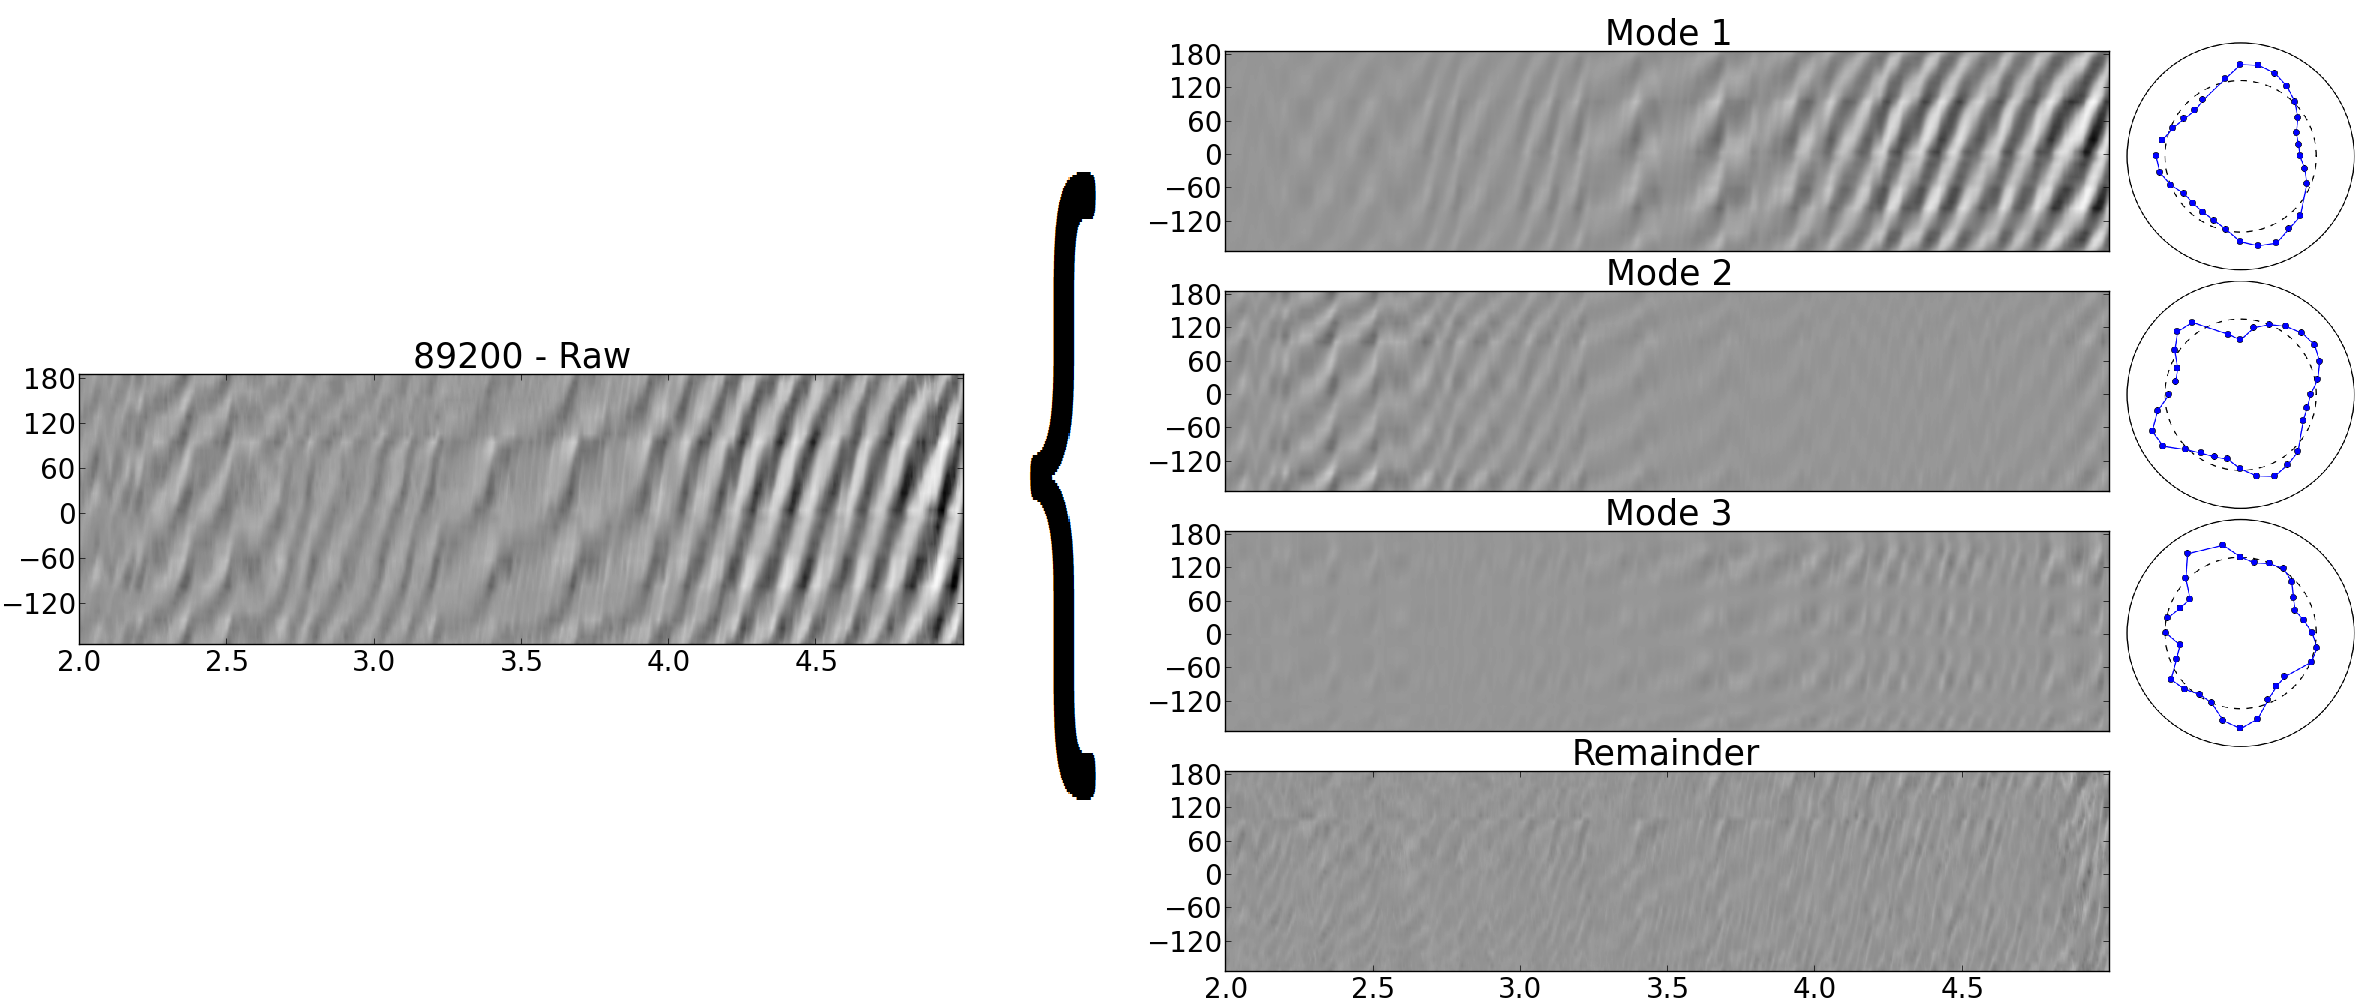
\includegraphics[width = \textwidth]{./figures/stripey_flucts_joined_grey_89200_mod.png}\begin{flushleft}
\caption{Left: contour plot of poloidal array raw signal, right: 3 dominant modes, and remainder of the full signal.  Mode structure is clearly visible, as is temporal evolution of mode amplitude.  Remainder shows structure - determining significance of low-order modes requires close analysis on a shot-by-shot basis}\label{fig:PA_sensors_top_3_modes}
\end{flushleft}
\end{figure}

\section{Equilibrium Subtraction}
\paragraph{}
Removing the background equilibrium prior to BD analysis for a real shot has been shown to be important for the purposes of isolating MHD modes.  This was previously done by either taking a sliding or 'boxcar' average of the signal, and treating the resulting time-smoothed signal as the equilibrium, or in certain situations, fitting a subset of the datapoints to a polynomial and then treating the polynomial as the equilibrium.  This is crucial for this research as the imposition of the shaping field significantly changes the equilibrium field near the X-point for sensors nearest the X-point. 